\documentclass[20pt]{extarticle}
\usepackage[]{geometry}

\def\pagewidth{1404}
\def\pageheight{1872}
\def\sidebarwidth{120}
\def\headerheight{80}
\def\incwidth{560}
\def\incheight{ 500 }
\def\paddinginner{ 40 }

\geometry{
  paperwidth=1404px,
  paperheight=1872px,
  margin=0px
}

\setlength{\parindent}{0pt}

\usepackage{tikz}
\usetikzlibrary{calc}
\usetikzlibrary{patterns,patterns.meta}
% \tikzset{
%   font={\fontsize{36pt}{36}\selectfont}}

\title{Ops Chart}
\date{}
\author{Nuno Casteleira}

\begin{document}


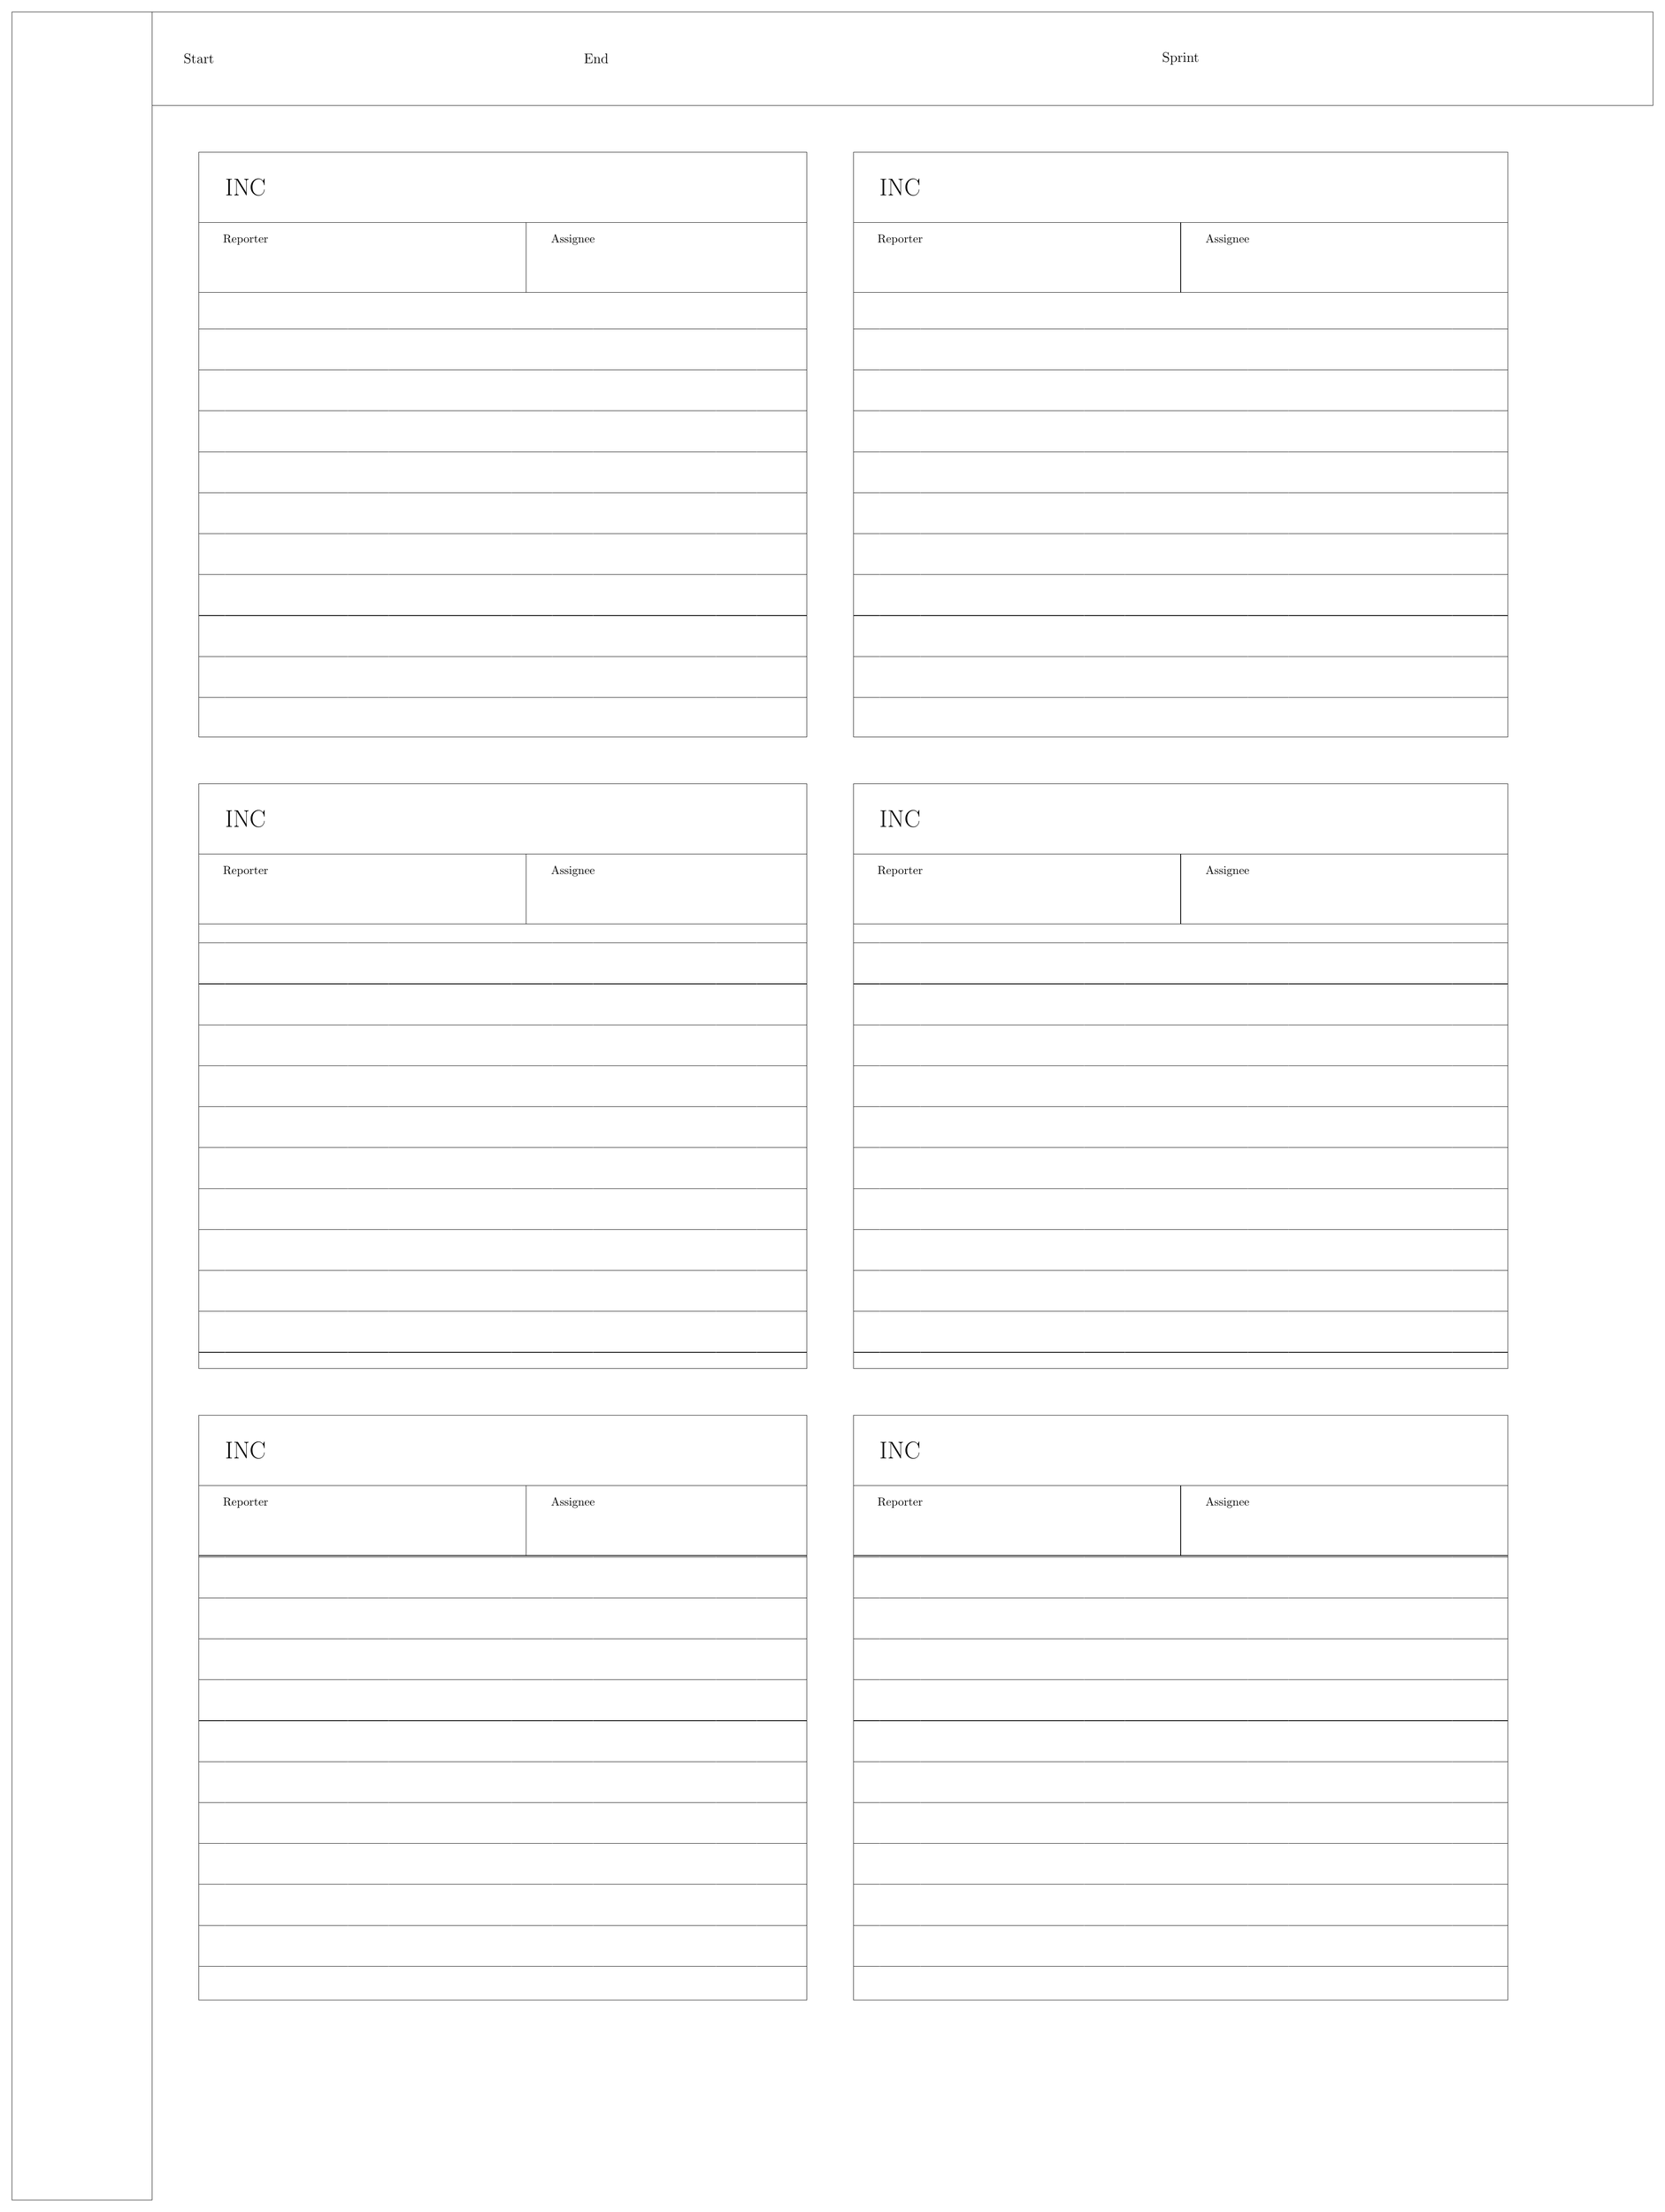
\begin{tikzpicture}[x=1px,y=1px]
  % \draw [help lines,xstep=50,ystep=50] (0,0) grid (1400,-1870);

  % Sidebar
  \draw (0,0) rectangle (\sidebarwidth,{(-1 * \pageheight) + 1});

  % Header
  \draw (\sidebarwidth,0) rectangle (\pagewidth,\headerheight * -1);
  \node at (160,-40) {\large Start};
  \node at (500,-40) {\large End};
  \node at (1000,-40) {\large Sprint};

  \def\incheaderheight{60}
  \foreach \I in {0,...,2}
  \foreach \J in {0,1}
  {
    % one incident
    \def\xleft{\sidebarwidth + \paddinginner + \J * \incwidth}
    \def\ytop{-1 * (\headerheight + (\I + 1) * \paddinginner + \I * \incheight)}

    \def\xright{\sidebarwidth + \J * \paddinginner + \incwidth + \J * \incwidth}
    \def\ybot{-1 * (\headerheight + (\I + 1) * \paddinginner + (\I + 1) * \incheight)}
    \draw (\xleft, {\ytop}) rectangle (\xright, {\ybot});

    \draw (\xleft, {\ytop - \incheaderheight}) --%
    (\xright, {\ytop - \incheaderheight});
    \node at (\xleft + 40, {\ytop - \incheaderheight + 30}) {\huge INC};

    \draw (\xleft, {\ytop - 2* \incheaderheight}) --%
    (\xright, {\ytop - 2 * \incheaderheight});
    \node at (\xleft + 40, {\ytop - 2 * \incheaderheight + 45}) {Reporter};

    \draw (\xleft + \incwidth / 2, {\ytop - \incheaderheight}) --%
    (\xleft + \incwidth / 2, {\ytop - 2 * \incheaderheight});
    \node at (\xleft + \incwidth / 2 + 40, {\ytop - 2 * \incheaderheight + 45}) {Assignee};


    \draw[pattern={Lines[distance={35px}],pattern color=black!30}]
    (\xleft, {\ytop - 2 * \incheaderheight}) rectangle (\xright,{\ybot});
  }

\end{tikzpicture}
\end{document}
